\begin{multicols*}{2}
	[\section{Introduction}]
	Product Development is driven by stakeholder requirements. The larger the developed system, the harder it is to analyze and verify it. Software Projects are no exceptions. This project aims to show how the verification of huge software projects can be performed automatically against the given requirements. The project spreads across multiple areas of main stream research.
	
	\begin{figure}[H]
		\centering
		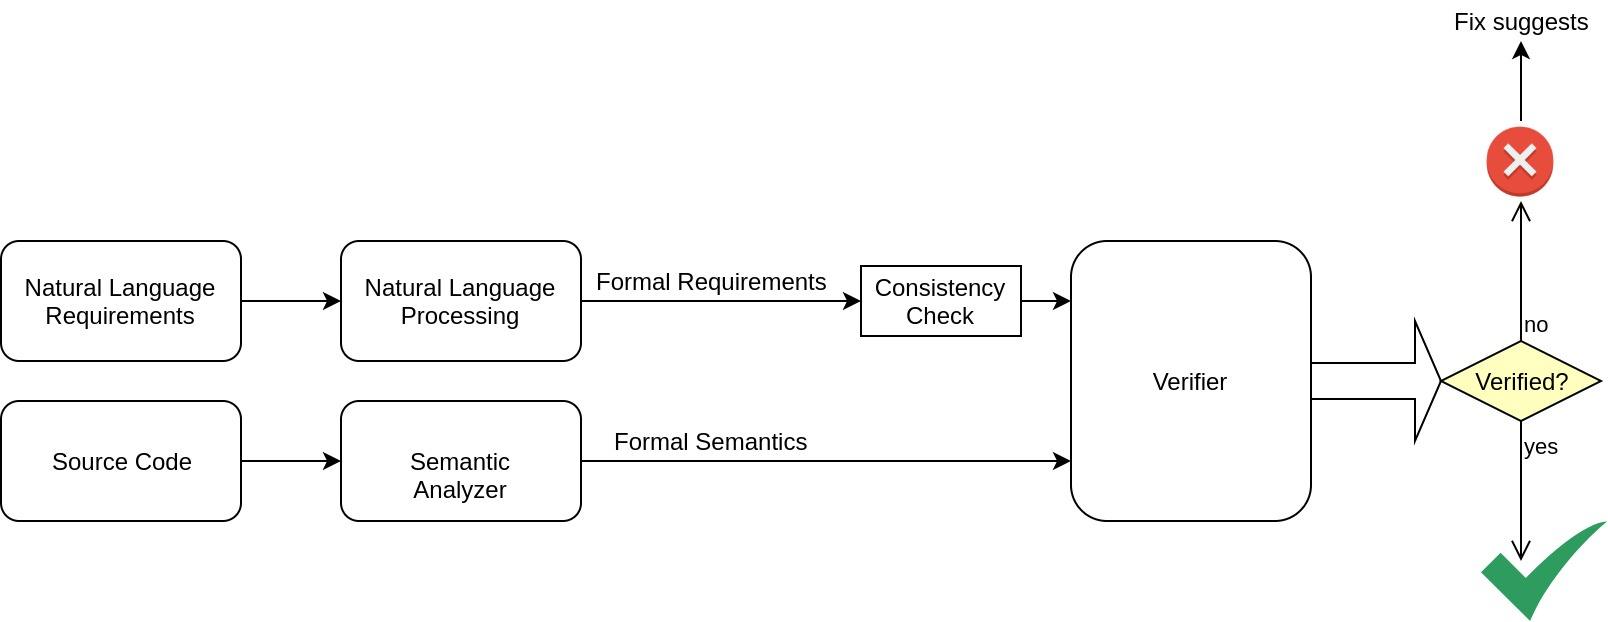
\includegraphics[width=1\linewidth]{../Architecture}
		\caption[PorjArch]{Project Architecture}
		\label{fig:architecture}
	\end{figure}
	
	\gls{NLP} is used for formalizing the \gls{SRS}. Since, natural language is widely understood by stakeholders, it is used as a common way for representing requirements. Representing requirements in natural language suffers from potential problems like ambiguity, inconsistency and incompleteness. A systematic literature review in the last two decades from 1995 till 2016 shows that collecting ambiguous requirements is one of the highest critical challenges in software engineering \cite{Besrour}. Since the advent of software engineering, researchers used formal and semi-formal methods to overcome this problem. However, even when formal and semi-formal languages are used, there is no escape from natural language as the initial requirements are written in natural language \cite{Kamsties}. The consequences of ambiguous requirements will lead to excessive efforts, high cost and failure in some software projects. For example, software developers might decide a subjective interpretation of requirements based on their point of view. Ferrari et al. (2014) argued that this subjective interpretation leads to designing software in a different way from what was intended in the requirements \cite{Ferrari}. For several decades, \gls{SRS} processing and analysis has been the focus of research in software engineering discipline. Since natural language is ambiguous, a computer cannot provide full support to analyze \gls{SRS} in an automatic fashion. Consequently, the analysis of \gls{SRS} is conducted manually which consumes time, effort and cost. Most importantly, the manual analysis of requirements results in inefficiency and imprecise results \cite{Wang}. The problem will be more obvious and critical when software projects involve thousands of requirements and hundreds of \gls{SRS} documents. Conducting verification of thousands of requirements via humans will become extremely expensive \cite{Fanmuy}. Generally, the primary source of problems in requirement engineering is reliance on humans extensively \cite{Ahmed}. This discussion leads to the importance of finding an automatic way for processing \gls{SRS}. \gls{NLP} was used as a possible solution to resolve ambiguity and to provide valuable information to the intended software developers. Ryan (1993) argued that: ”It is highly questionable that the resulting system from \gls{NLP} would be of great use in requirements engineering” \cite{Ryan}. Nazir et al. (2017) conducted a systematic literature review on \gls{NLP} applications for software requirement engineering, he concluded that: “Manual operations are still required on initial plain text of software requirements before applying the desired \gls{NLP} techniques” \cite{Nazir}.
	
	On the other hand the formal semantics of the source code is needed.  A formal semantics should serve as a solid foundation for any programming language development, so it must be correct and complete (to be trusted and useful), executable (to yield a reference implementation), and appropriate for program reasoning and verification.
	
	The five most popular programming languages according to GitHub in 2019 is JavaScript, Python, Java, PHP and C\#. Several efforts to give JavaScript a formal semantics have been made, most notably by Politz et al. \cite{Politz} and Bodin et al. \cite{Bodin}. But Unfortunately, these address fragments of the language and are not fully validated with a formal JavaScript semantics. Having to define two or more different semantics for a real-life language, together with proofs of equivalence, is a huge burden in itself, not to mention that these all need to be maintained as the language evolves. Due to the functional nature of their interpreters, these semantics cannot handle the nondeterminism of JavaScript well. Finally, their interpreters are not suited for symbolic execution, and thus for developing program reasoning tools.
	
\end{multicols*}

